\subsubsection{Signal Processes}
\label{sec:signal}
The signal processes studied in this analysis 
%\- tells it where to break the line
are  $pp\rightarrow\- \Wp\Wp\Wm+X$ and $pp\rightarrow \Wp\Wm\Wm\allowbreak +X$, 
where $X$ is intended to refer to the fact that
no requirements are placed on additional particles produced in the hard
interaction.
The process includes associated Higgs production, 
or ``Higgsstrahlung'', where a $W$ boson radiates a Higgs boson,
$pp\rightarrow WH$, and subsequently decays into a $\Wp\Wm$ pair.
The Higgs decay results in one $W$ boson being produced off-shell,
$H\rightarrow WW^*$, making this the leading contribution to off-shell
production.  The resonance from the Higgs can clearly be seen from the 
distribution of $m_{\Wp\Wm}$ taken from simulation of \www~events
in \fig\ref{fig:mww_higgs}.
The \www process also includes contributions from 
the $WWWW$ quartic coupling. %and...?

%It would be nice to show a plot of the higgs stuff. maybe I can
%steal this and make my own later...
\begin{figure}[ht]
\centering
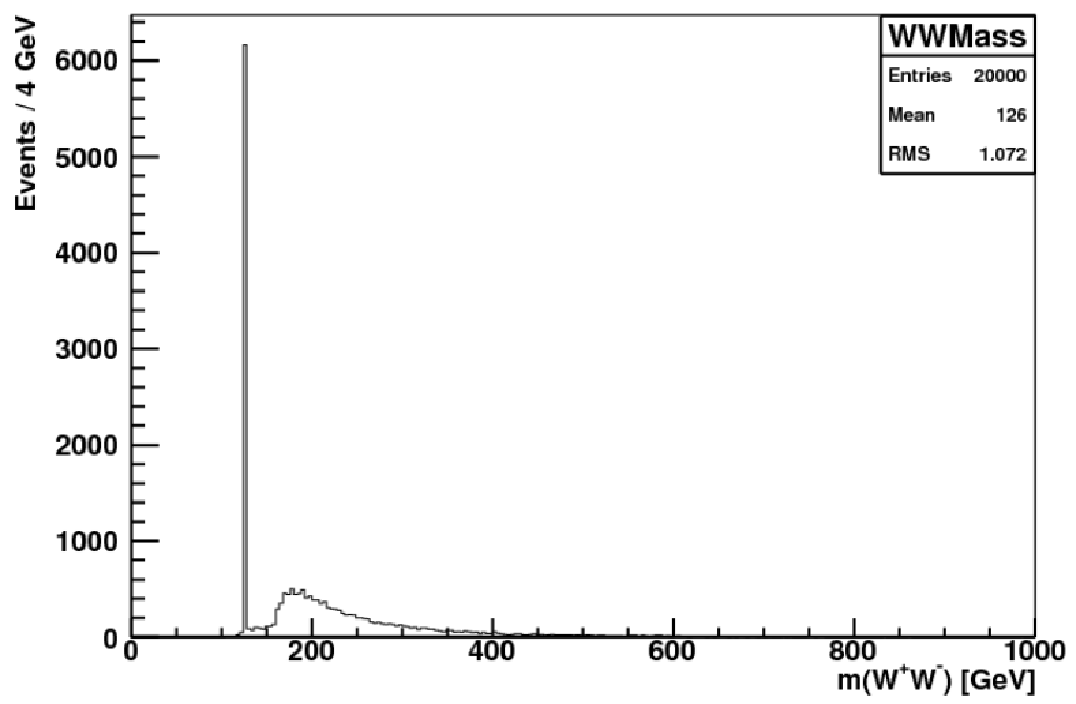
\includegraphics[width=0.5\columnwidth]{figures/2l2j/mWW-parton.pdf}
\caption{ Invariant mass distribution of two opposite-sign $W$ bosons 
in \www events generated with VBFNLO at LO. The Higgs mass peak is clearly 
visible at 126~GeV.}

\label{fig:mww_higgs}
\end{figure}


%%%
%If I'm going to include this, I better read up on it.
%%%
%The production \xsec without Higgs contribution has been calculated 
%to $\mathcal{O}(\alpha_s)$  corrections in ref~\cite{Binoth:2008kt}.
%$\mathcal{O}(\alpha_s)$ corrections, Higgs boson exchange and spin 
%correlations of $W$ bosons lepton decay are also available
%~\cite{Campanario:2008yg}.  

The SM signal processes are implemented in the Monte
Carlo generator \vbfnlo~\cite{Arnold:2011wj,Arnold:2012xn},
which can generate partonic events at leading-order (LO) with
next-to-leading-order (NLO) cross-sections, 
and in \madgraph~\cite{MadGraph}, which can generate
partonic events at NLO with NLO cross-sections. 
The partonic events are further processed 
by \pythiaeight\cite{Sjostrand:2007gs} and \photos\cite{Golonka:2005pn} 
to add effects of beam remnant interactions and initial and 
final state radiation. 
SM parameters must be provided to the MC generators as input. 
The most relevant input parameters are listed 
for the generators in \tab\ref{tab:signal_sm_parameters}.
The parameters are set in \pythiaeight using the ATLAS tune 
of AU2\cite{ATLAS:2011zja}.
The MC generators must also be provided an appropriate PDF.
The PDF used  in the LO \vbfnlo~generation is
the LO CTEQ6L1~\cite{Pumplin:2002vw} PDF set 
while CT10 NLO~\cite{Guzzi:2011sv}
is used in the NLO \vbfnlo~cross-section calculation.
The PDF used in the NLO \madgraph~generation 
and \xsec~calculation is CTEQ6L1 
but this is reweighted to CT10 NLO using a k-factor.
Since the MC generators are computed to finite order in perturbation
theory, renormalization and factorization scales must be chosen.
The renormalization and factorization scales are dynamically
set to the $WWW$ invariant mass in the \vbfnlo~samples, while they 
are set to a fixed scale equal to the $Z$ mass in \madgraph.
The \vbfnlo~samples are restricted to leptonic decays of the $W$~bosons
where each lepton has a \pt~of at least 5~\GeV. Meanwhile, the \madgraph~
samples include all decays of the $W$~boson, with a requirement 
that jets have a a \pt~of at least 10~\GeV but with no requirement
on the \pt~of leptons.
The \vbfnlo~ and \madgraph~samples handle interference 
between $WH\rightarrow WWW(*)$ 
and on-shell $WWW$ production at LO, but \madgraph~is not
able to do this at NLO. As a result, the NLO \madgraph~samples
are split by on-shell \www~ and $WH\rightarrow WWW(*)$ production.
Both sets of samples are further split by the \www charge mode.
For each sample, The \xsecs are summarized in \tab\ref{tab:signal_xsec} 
in their full phase space and in a common fiducial phase space
defined in \sec...  The fiducial \xsecs are observed to be nearly the same
between the two generators,
as expected.  This serves as a good check of the understanding of the 
signal process. The \madgraph~\xsecs are used throughout the 
remainder of the analysis.

%Do I need to describe the k-factors?
%It would be nice to also add some distributions from Rivet comparing
%the two at truth level.


%Describe the pdf uncertainty calculation.
%what about renormalization and factorization scales




\begin{table}[ht]
\centering
\begin{tabular}{|l||c|c||}
\hline
 & \vbfnlo & \madgraph \\
\hline
\hline
Higgs mass, $m_H$ & 126.0~\GeV & \\ 
Top mass, $m_t$ & 172.4~\GeV  & \\
$Z$ mass, $m_Z$ & 91.1876~\GeV & 91.188~\GeV\\
$W$ mass, $m_W$ & 80.398~\GeV & \\
Fermi constant, $G_F$ & $1.16637\times 10^{-5}~\GeV^{-2}$ & \\
\hline
\end{tabular} 


\caption{List of the most relevant SM parameters used as input to the 
signal MC generation.}
\label{tab:signal_sm_parameters}
\end{table}


\begin{table}[ht]
\centering
\begin{tabular}{|cc||c|c|c|}
\hline
\multicolumn{2}{|c||} {Sample} &  \multicolumn{2}{c|}{Cross-section [fb]} \\
                              && Inclusive & Fiducial \\
\hline
\hline
%\multirow{3}{*}{\vbfnlo~LO} & $W^{+}W^{+}W^{-}\rightarrow l\nu l\nu l\nu$ & $3.56 \pm 0.005$ & \\
%                            & $W^{-}W^{+}W^{-}\rightarrow l\nu l\nu l\nu$ & $1.88\pm0.003$ & \\ 
%			    \cline{2-4} 
%                            & Sum & $5.44\pm0.006$ & \\ 
%\hline
\multirow{3}{*}{\vbfnlo~NLO} & $W^{+}W^{+}W^{-}\rightarrow l\nu l\nu l\nu$ & $4.95 \pm 0.007$ & $0.2050 \pm 0.0070$\\
                           & $W^{-}W^{+}W^{-}\rightarrow l\nu l\nu l\nu$ & $2.65\pm0.004$ & $0.0987 \pm 0.0037$\\ 
			    \cline{2-4} 
                           %& $WWW\rightarrow l\nu l\nu l\nu$ & $7.60\pm0.008$ & \\ 
                           & Sum & $7.60\pm0.008$ & $0.3037 \pm 0.0072$\\ 
\hline
%With PDF KFactor
\multirow{5}{*}{\madgraph~NLO} & $W^{+}W^{-}W^{+}\rightarrow \textrm{Anything}$ &$59.47\pm0.11$ & $0.0900 \pm 0.0048$\\
                        & $W^{-}W^{+}W^{-} \rightarrow \textrm{Anything}$& $28.069\pm0.076$ & $0.0476 \pm 0.0043$\\
                        & $W^{+}H\rightarrow W^{+}W^{+}W^{-}(*)\rightarrow\textrm{Anything}$ & $99.106\pm0.019$ & $0.1114 \pm 0.0029$\\
                        & $W^{-}H\rightarrow W^{-}W^{+}W^{-}(*) \rightarrow \textrm{Anything}$& $54.804\pm0.010$ & $0.0603 \pm 0.0015$\\
			\cline{2-4} 
                        & Sum & $241.47\pm0.13$ & $0.3092 \pm 0.0072$\\
%Without PDF KFactor
%\multirow{5}{*}{\madgraph~NLO} & $W^{+}W^{-}W^{+}\rightarrow \textrm{Anything}$ &$55.07\pm0.10$ & $0.0818 \pm 0.0044$\\
%                        & $W^{-}W^{+}W^{-} \rightarrow \textrm{Anything}$& $25.99\pm0.07$ & $0.0433 \pm 0.0039$\\
%                        & $W^{+}H\rightarrow W^{+}W^{+}W^{-}(*)\rightarrow\textrm{Anything}$ & $91.765\pm0.018$ & $0.1013 \pm 0.0026$\\
%                        & $W^{-}H\rightarrow W^{-}W^{+}W^{-}(*) \rightarrow \textrm{Anything}$& $50.7440\pm0.0094$ & $0.0548 \pm 0.0014$\\
%			\cline{2-4} 
%                        & Sum & $223.57\pm0.12$ & $0.2812 \pm 0.0066$\\
\hline
\end{tabular}

\caption{Inclusive and common fiducial cross-sections at NLO 
for \vbfnlo~and \madgraph~samples. 
The sum of the inclusive \xsecs are different
because of the different branching fractions in the two cases. However,
the sum of the fiducial \xsecs are expected to be similar because
they are computed for the same phase space, as described in \sec...}
\label{tab:signal_xsec}
\end{table}


%%%%
%soud I show the dependence on scales here?
%%%%
%The dependencies of the 
%$\xsecs on the choices of scales have been studied in the two
%references~\cite{Binoth:2008kt,Campanario:2008yg}. 

% The production at LO is a pure electroweak process. The
% NLO correction brings in $\alpha_s$ which actually makes the cross
% sections more sensitive to the choices of scales. 
%It has been pointed
%out that a jet veto should reduce the scale dependence. 

%The $W$ boson is short lived, so one must study its decay products.
%As already mentioned, the focus of this analysis is on the final state 


%need to also show the madgraph parameters
%maybe repphrase so that I can discuss both in parallel
%get generation parameters from semi-leptonic note
%report both sets of cross-sections here
%include updated info on cross-sections and pdfs 

\begin{figure}[ht!]
\centering
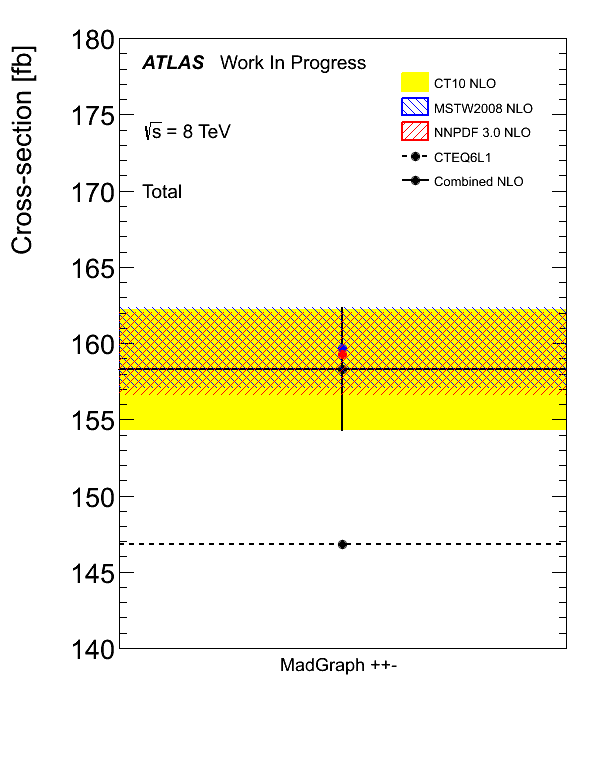
\includegraphics[width=.35\columnwidth]{figures/pdf/MADppm_total_cteq6l1.png}
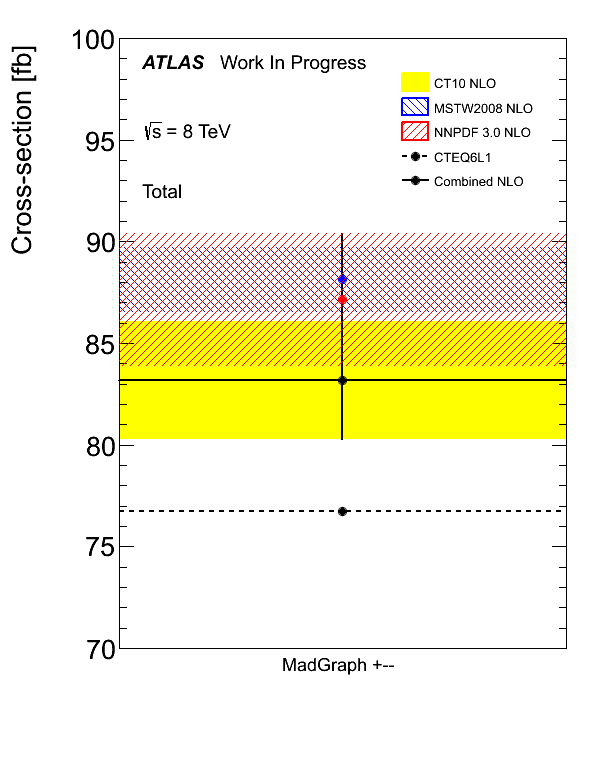
\includegraphics[width=.35\columnwidth]{figures/pdf/MADpmm_total_cteq6l1.png}
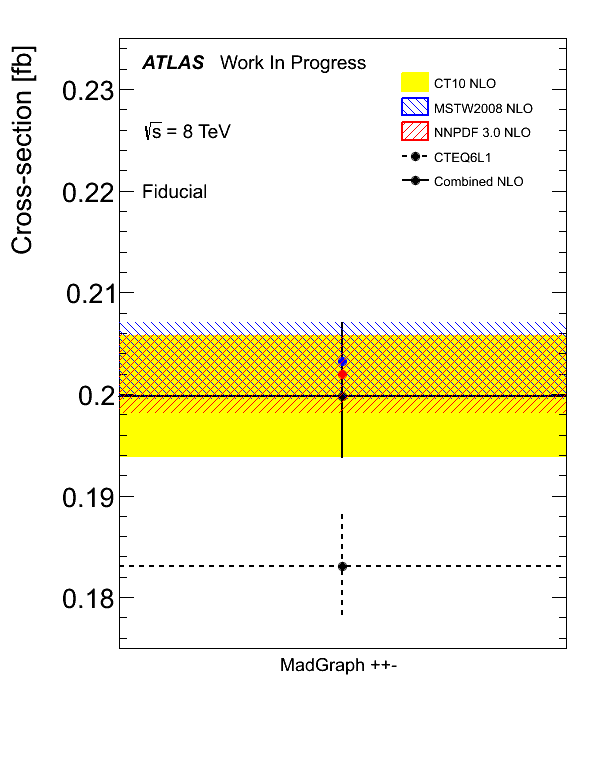
\includegraphics[width=.35\columnwidth]{figures/pdf/MADppm_fiducial_cteq6l1.png}
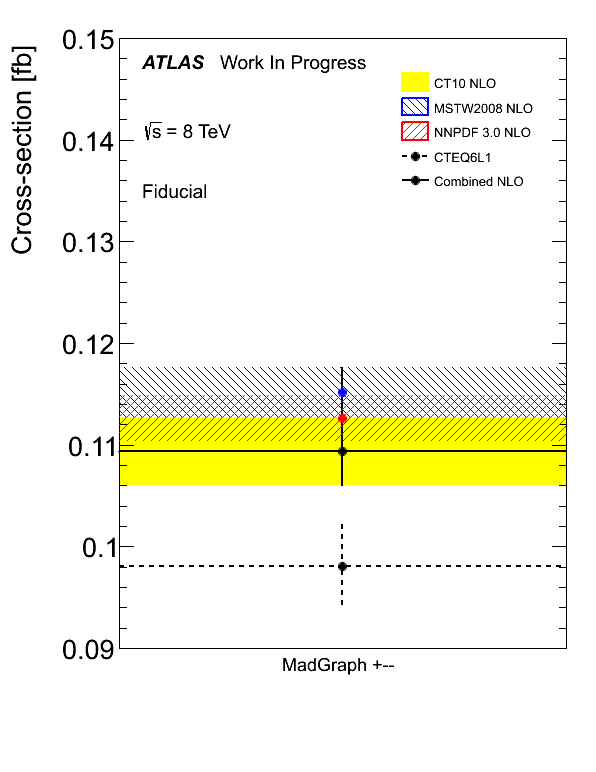
\includegraphics[width=.35\columnwidth]{figures/pdf/MADpmm_fiducial_cteq6l1.png}
\caption{The signal cross-sections for different PDFs along with their
uncertainties are shown on the {\sc MadGraph} $WWW$ signal samples
for the total $WWW$ phase space and branching fraction for
for the $W^{+}W^{+}W^{-}$ (top left) and $W^{+}W^{-}W^{-}$ (top right)
charge modes
and in the fiducial region for $W^{+}W^{+}W^{-}$ (bottom left) 
and $W^{+}W^{-}W^{-}$ (bottom right).
The bands show the PDF uncertainty for CT10 NLO (solid yellow),
MSTW 2008 NLO (hashed blue), and NNPDF 3.0 NLO (hashed red) while the
solid line shows the envelope of all uncertainty bands used as the final
PDF uncertainty estimate. The central value of CT10 NLO is taken as the
central value of the estimate.
The dashed-line shows the cross-section and 
statistical uncertainty for the CTEQ6L1
pdf sets used in the original generation step.}
\label{fig:signal_pdf_unc}
\end{figure}

\begin{table}[ht!]
\centering
\begin{tabular}{c|c|c}
\hline
 & \multicolumn{2}{c}{PDF Uncertainty}\\
 & $W^{+}W^{+}W^{-}$ & $W^{+}W^{-}W^{-}$ \\
\hline
\hline
Total & $+2.58\%~-2.51\%$ &  $+8.69\%~-3.47\%$ \\
Fiducial & $+3.64\%~-3.00\%$ & $+7.57\%~-3.08\%$ \\
\hline
\end{tabular}
\caption{Summary of PDF uncertainties estimated on NLO {\sc MadGraph} cross-sections
in both the fiducial and total phase space.}
\label{tab:pdfunc}
\end{table}

The uncertainty on the PDF is derived for the {\sc MadGraph} 
cross-sections following a modified version of the pdf4lhc
\cite{Botje:2011sn} recommendations.  The resulting 
uncertainty is shown separately for the two different charge modes
in both the fiducial and the inclusive phase
space in Table~\ref{tab:pdfunc}.
The uncertainty is determined by comparing three different PDFs;
CT10 NLO~\cite{Lai:2010vv}, MSTW2008 NLO~\cite{Martin:2009iq}, 
and NNPDF 3.0 NLO~\cite{Ball:2014uwa}. 
This comparison is presented in Figure~\ref{fig:signal_pdf_unc}.  
Symmetric 68\%CL uncertainties 
are determined for CT10 NLO and MSTW 2008 NLO using the 68~\% CL 
set provided for MSTW and the 90~\%CL for CT10 and scaling down by 
the factor 1.645. The uncertainty of the NNPDF 3.0 NLO PDF is 
determined by using the standard deviation of the distribution 
of 101 MC PDFs provided in the PDF set while the nominal value is taken
from the mean of the same PDFs.  
The CT10 NLO PDF central value is used as the nominal 
value of the final estimate
while the final PDF uncertainty on that estimate is
taken as the envelope of the uncertainty bands for all three PDF sets.  



The uncertainty on the factorization and renormalization scales are 
determined by varying each of them independently up or down by 
a factor of two. 
The effect of these variations on the cross-sections
as compared to the nominal
are shown separately for the two different charge 
modes in \tab~\ref{tab:scaleVariation}.
The uncertainty is then determined by taking the maximum 
variation for each charge mode, 
namely, 2.62\% for $W^+W^+W^-$ and 2.53\% for $W^-W^+W^-$. 

\begin{table}[ht!]
    \centering
\begin{tabular}{cc|ccc}
\hline
& \backslashbox{$\mu_F$}{$\mu_R$}     & $\frac{1}{2}M_{WWW}$ & $M_{WWW}$ &  $2M_{WWW}$ \\
\cline{2-5}
\multirow{3}{*}{\Wp\Wp\Wm} &$\frac{1}{2}M_{WWW}$ & 2.62\% & -0.14\% & -2.11\% \\
%\cline{2-5}
&$M_{WWW}$ & 2.13\% & 0 & -2.41\% \\
%\cline{2-5}
&$2M_{WWW}$ & 1.56\% & 0.24\% & -2.42\% \\
\hline
\hline
& \backslashbox{$\mu_F$}{$\mu_R$}     & $\frac{1}{2}M_{WWW}$ & $M_{WWW}$ &  $2M_{WWW}$ \\
\cline{2-5}
\multirow{3}{*}{\Wm\Wp\Wm} &$\frac{1}{2}M_{WWW}$ & 1.91\% & 1.38\% & -2.00\% \\
%\cline{2-5}
&$M_{WWW}$ & 1.61\% & 0 & -2.53\% \\
%\cline{2-5}
&$2M_{WWW}$ & 1.25\% & -1.05\% & -2.12\% \\
\hline
\end{tabular}
\caption{The relative variation of the NLO cross sections corresponding 
to different choices of factorization and renormalization 
scales for the \Wp\Wp\Wm and \Wm\Wp\Wm  processes. }
\label{tab:scaleVariation}
\end{table}

The signal cross-sections and uncertainties are thus determined to be 
\begin{equation}
\sigma^{\textrm{Total}}_{\textrm{Theory}}= 241.47\pm0.13 ~(\textrm{Stat.}) ~^{+10.33}_{-6.08} ~(\textrm{PDF}) ~\pm 6.3 ~(\textrm{Scale}) ~\textrm{fb} %uncertainty?
\end{equation}
for the inclusive \xsec and
\begin{equation}
\sigma^{\textrm{Fiducial}}_{\textrm{Theory}}= 309.2\pm7.2 ~(\textrm{Stat.}) ~^{+15.05}_{-8.36} ~(\textrm{PDF}) ~\pm 8.0 ~(\textrm{Scale}) ~\textrm{ab} %uncertainty?
\end{equation}
for the fiducial cross-section.


%should i include this
%The analysis considers events with three leptons ($e$ or $\mu$) in the final state. The contributions from events in which $W$ bosons decay to $\tau$'s, and the $\tau$'s sequentially decay to $e$ or $\mu$ should be included and is expected to be 40\% of total yield of the 3-lepton final state.  


\subsubsection{aQGC signal}
need to update 
%
MC samples of the aQGC signal processes described in \sec\ref{sec:eft}
have been generated using \vbfnlo at NLO in QCD.  (but don't we use LO?)
The cross-sections for the aQGC signal depend on the values
of the couplings $f_{s,0}$ and $f_{s,1}$. MC samples have 
been generated for a grid of points in the $f_{s,0}$ vs $f_{s,1}$ space
and their cross-sections are shown in \fig\ref{fig:aqgc_total_xsec_ununitarized_3l}. %histogram of cross-sections

\begin{figure}[ht!]
\centering
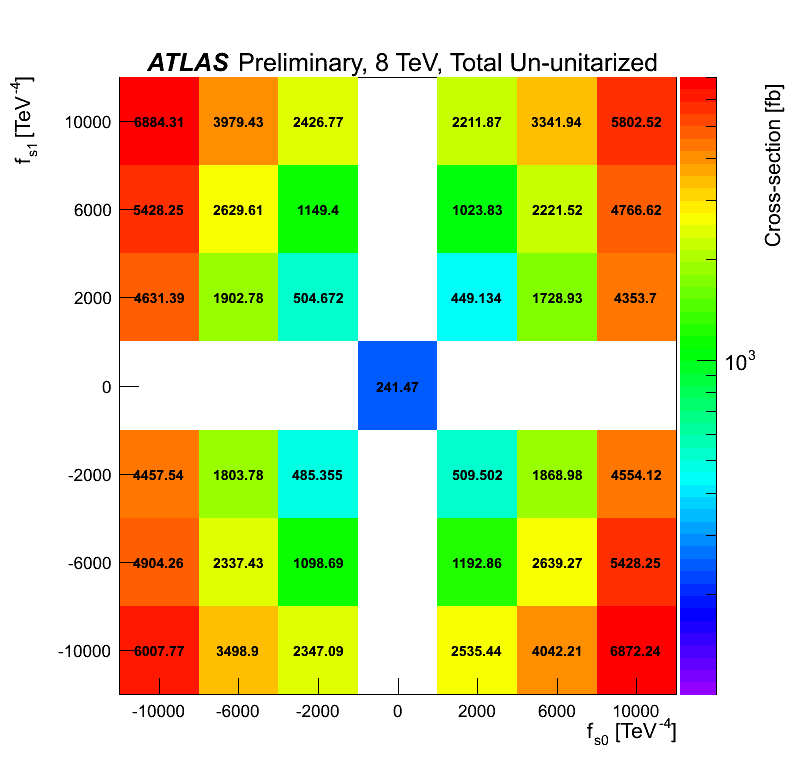
\includegraphics[width=.8\textwidth]{figures/aQGC/total_xsec/www_3l_aqgc_total_ununitarized_noratio.png}
\caption{Total cross-section for non-unitarized aQGC signal samples as a function of $f_{s,0}$ vs $f_{s,1}$.
The total SM cross-section is shown at $f_{s,0}=f_{s,1}=0$ for comparison.}
\label{fig:aqgc_total_xsec_ununitarized_3l}
\end{figure}

The issues of unitarity violation \sec\ref{sec:eft} are taken
into account using a form factor like in \eqn\eqref{eq:form_factor}.
The choices of the exponent, $n$, and form factor scale, $\Lambda$, 
are somewhat ad-hoc. Furthermore, a complete study of the unitarity
behavior of this process has never been performed, so there are not
currently detailed prescriptions on what to choose. 
However, based on discussions with the authors of \vbfnlo, who
are at the moment trying to perform these studies, an exponent
of $n=1$ is expected to be sufficient to achieve unitarity 
for this process.  As for the choice of $\Lambda$, we have
chosen to look at a few different values, which cover a wide
range but which should follow a smooth interpolation. 
This has the advantage of providing information about the
sensitivity to the form factor that can be interpreted 
by theorists as they see fit. Dedicated MC samples
are generated with the unitarization applied for values
of $\Lambda =$ 500~\GeV, 1000~\GeV, 2000~\GeV, and 3000~\GeV.
The cross-sections for each of these unitarization cases
are shown in \fig\ref{fig:aqgc_total_xsec_unitarized_3l}.

\begin{figure}[ht!]
\centering
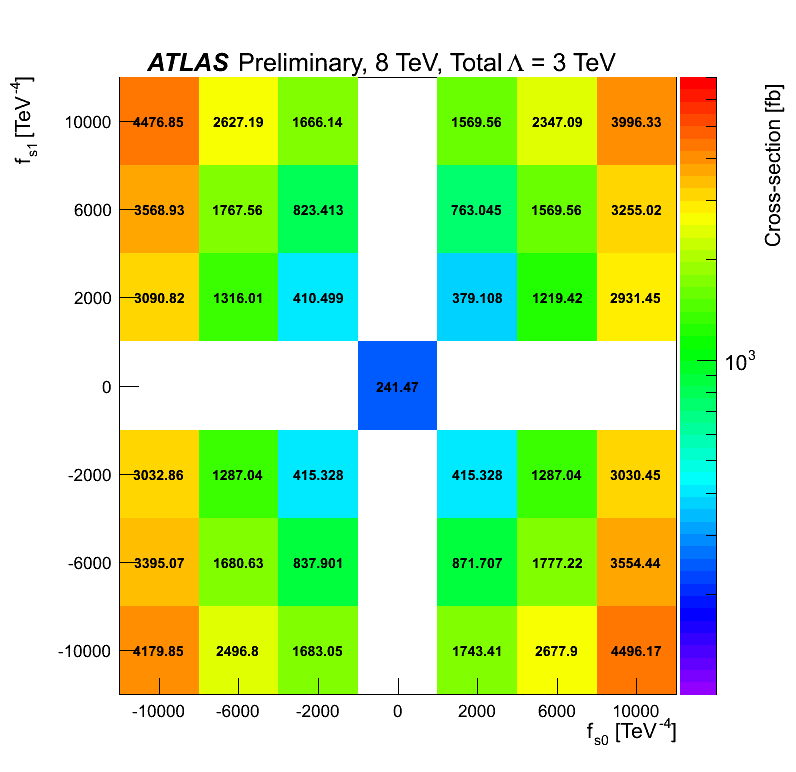
\includegraphics[width=.45\textwidth]{figures/aQGC/total_xsec/www_3l_aqgc_total_3TeV_noratio.png}
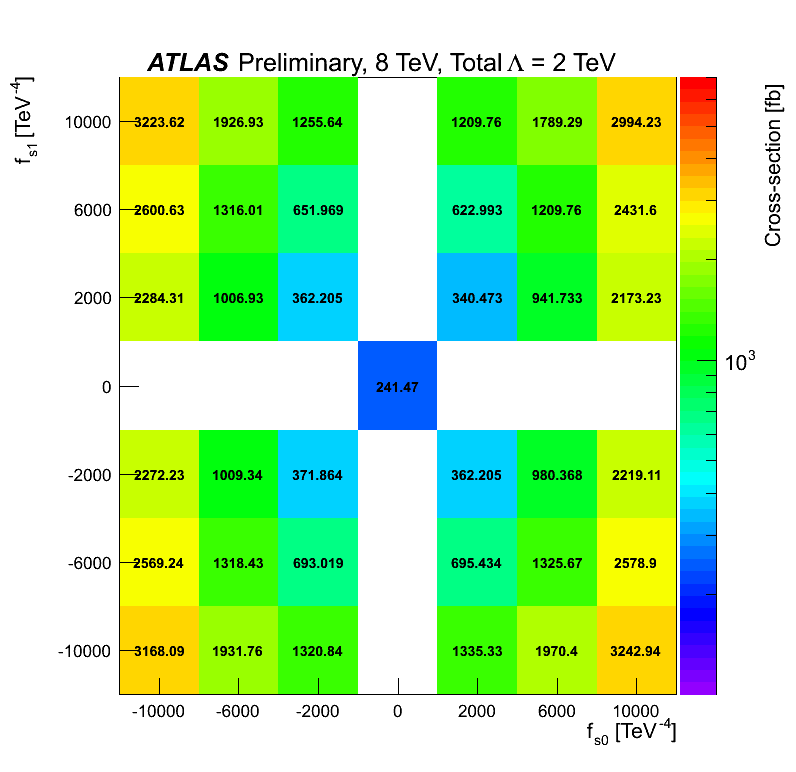
\includegraphics[width=.45\textwidth]{figures/aQGC/total_xsec/www_3l_aqgc_total_2TeV_noratio.png}
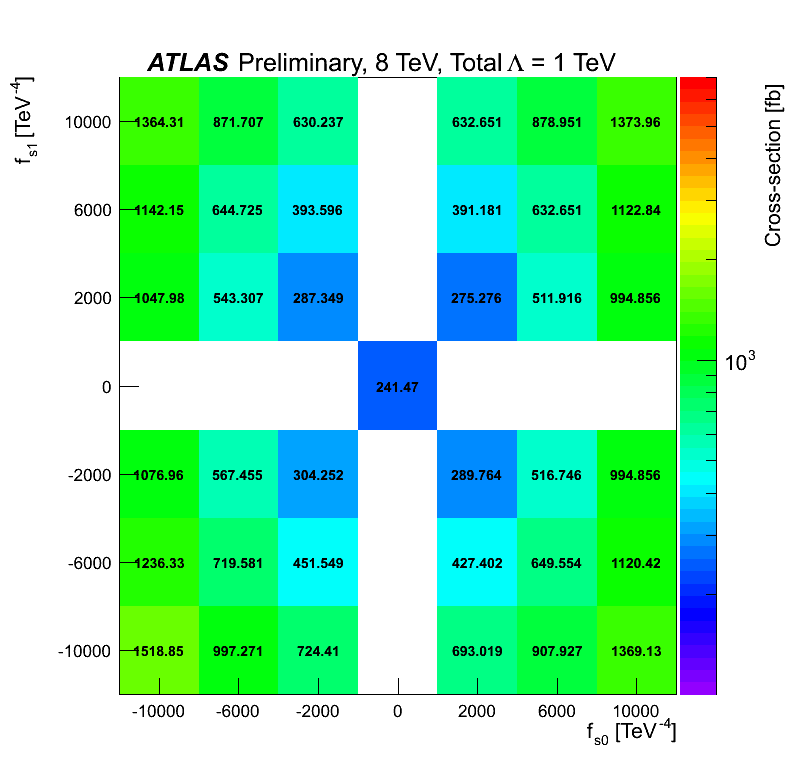
\includegraphics[width=.45\textwidth]{figures/aQGC/total_xsec/www_3l_aqgc_total_1TeV_noratio.png}
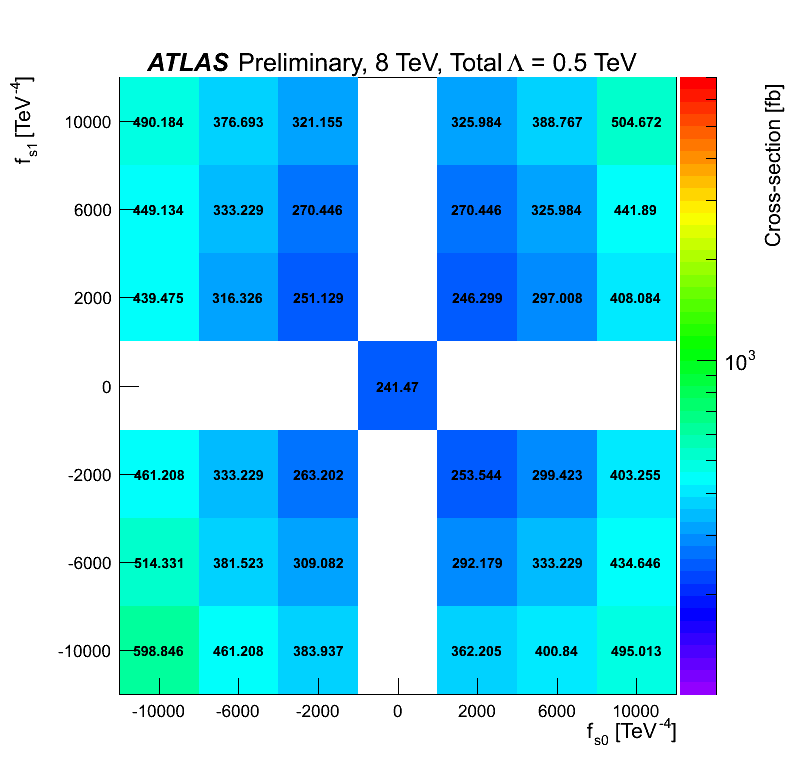
\includegraphics[width=.45\textwidth]{figures/aQGC/total_xsec/www_3l_aqgc_total_p5TeV_noratio.png}
\caption{Total cross-section for unitarized aQGC signal samples as a function of $f_{s,0}$ vs $f_{s,1}$.
Four different values of the unitarization scale, $\Lambda$, are chosen: 3~\TeV~(Top Left),
2~\TeV~(Top Right), 1~\TeV~(Bottom Left), and 0.5~\TeV~(Bottom Right).
The total SM cross-section is shown at $f_{s,0}=f_{s,1}=0$ for comparison.}
\label{fig:aqgc_total_xsec_unitarized_3l}
\end{figure}























